\section{Switchless Architecture}
\label{sec:arch}

The switchless architecture, as the name implies, removes switches from the data center network architecture.  Instead, switches are integrated into servers and the topology is chosen to keep the fanout of the in-server switches low.  The in-server switches could be implemented as separate boards attach to the server's I/O bus or they could be directly integrated with the processor on die.  We choose to focus on integrating the switches with the processor on die since silicon area is cheap and the latency from the processor to the switch is lower (and we are computer architects!).  In the following subsections, we discuss switchless network topologies, the design of in-server switches, the switchless network stack, and the benefits that come with the switchless architecture.

\subsection{Switchless Network Topologies}

We focus on two switchless network topologies, torus and cube.  The torus topology, Figure~\ref{fig:switchless_arch_torus}, is a two-dimensional topology where nodes are placed in a two-dimensional grid and are connected in all directions (north, south, east, and west).  Nodes at the edges have links that wrap around to the node at the opposite edge.  This creates a mesh fabric of nodes.  The cube topology, Figure~\ref{fig:switchless_arch_cube}, is similar to the torus topology with one additional dimension.  Nodes are placed into a three-dimensional grid and are also connected in all directions.  The cube topology with the same number of nodes as a given torus topology has higher bandwidth and lower average latency since nodes have more neighbors and the maximum hop count is lower.

One consideration when designing a data center network topology is wiring complexity.  While complex wiring is not a fundamental problem, it can affect the time and cost to setup the data center as well as the link length.  There is a tradeoff between bandwidth and cost of a link when considering link length.  Longer links are required to either be lower bandwidth or require a different link.  The bandwidth requirement of long links can be met by using thicker cabling or different cable technologies, such as optical links.  These links, however, are more expensive.

The cube topology actually maps well to a data center as far as wiring goes.  If racks are arranged in a two-dimensional grid, you can think of each layer of nodes in the racks as a torus.  A cube can be created by connecting the tori vertically.  Thus, the wiring is rather trivial.  A torus topology does not map as well to the data center, so the wiring may be more complex.  However, as mentioned earlier, this problem is not fundamental and can be solved.

\begin{figure}
    \centering
    \subfloat[Torus]
    {
        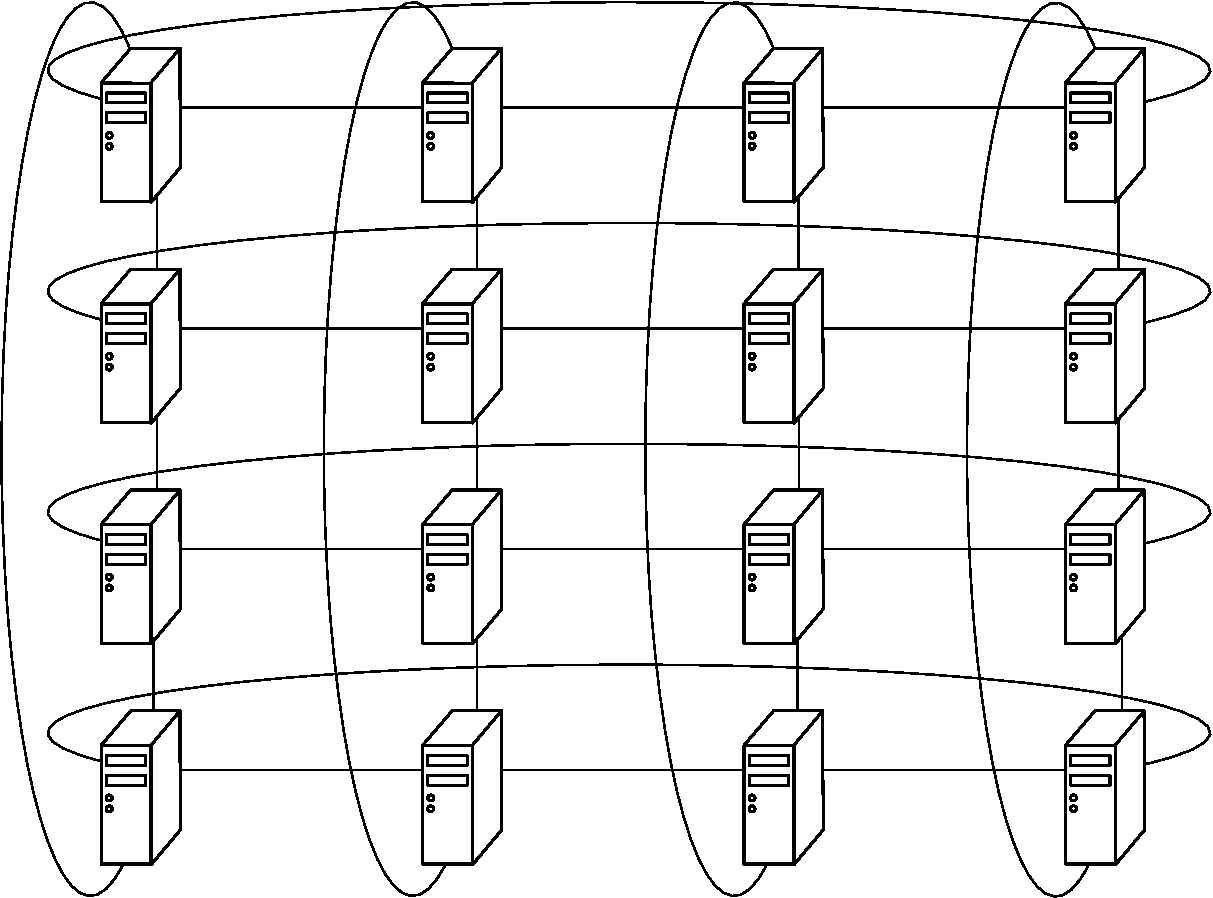
\includegraphics[width=0.2\textwidth]{switchless-arch-torus}
        \label{fig:switchless_arch_torus}
    }
    \\
    \vspace{-0.05in}
    \subfloat[Cube]
    {
        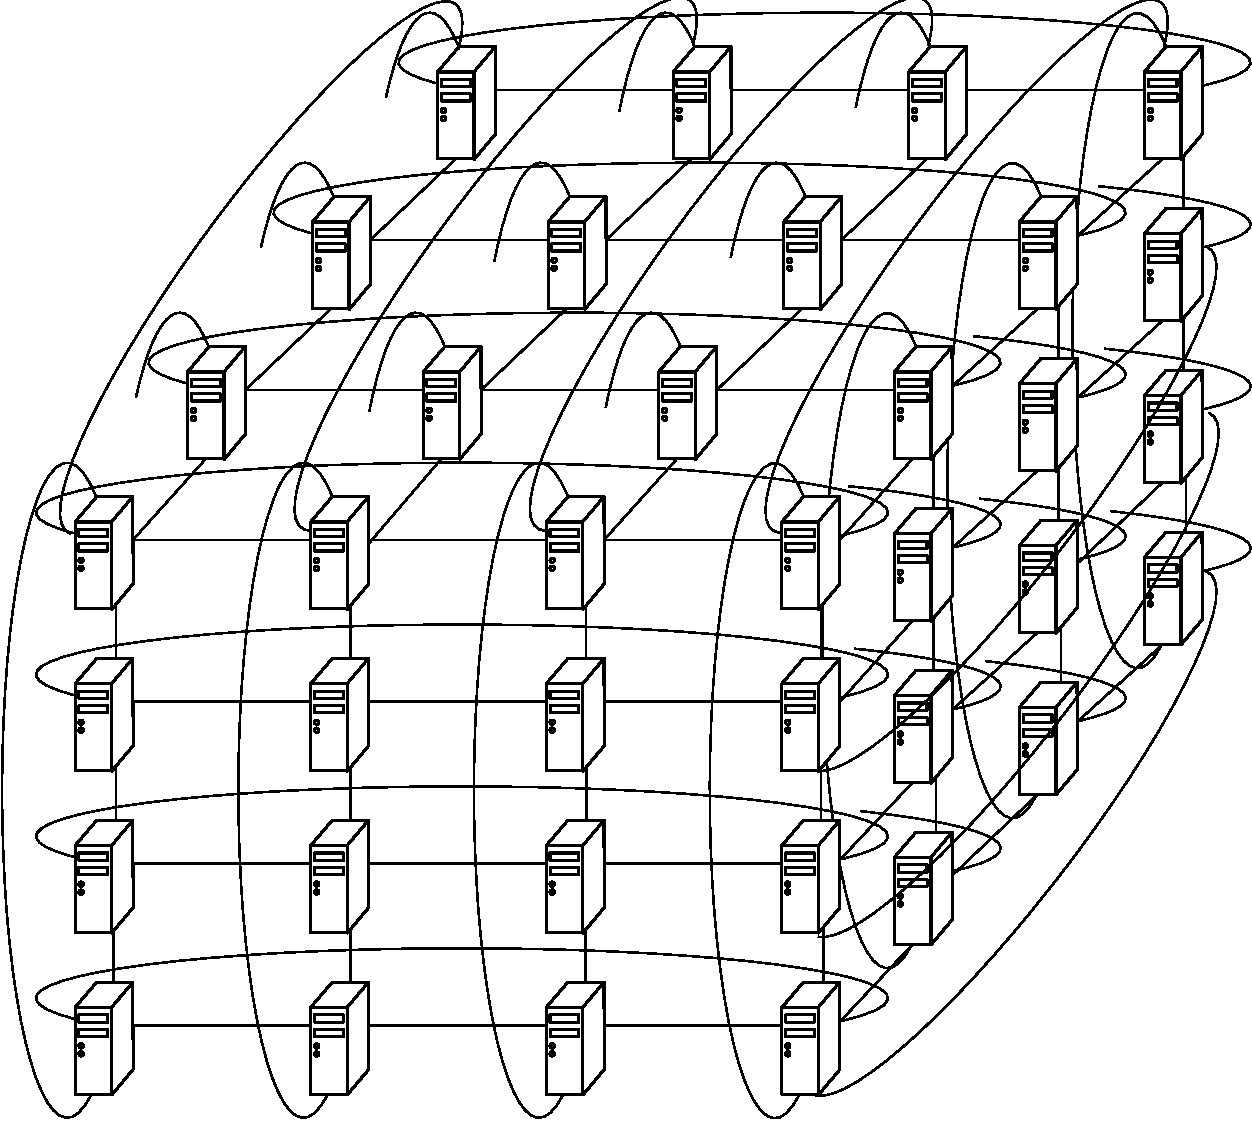
\includegraphics[width=0.25\textwidth]{switchless-arch-cube}
        \label{fig:switchless_arch_cube}
    }
    \vspace{-0.07in}
    \caption{Switchless Data Center Network Topologies}
    \label{fig:switchless_topos}
\end{figure}

\subsection{In-Server Switch Design}

We focus on integrating the switch with the processor on die.  As was mentioned previously, this is beneficial because silicon area is cheap and the latency from the processor to the switch is lower.  

Change in Topology
Removal of Switch
Change in Routing
Implementation Details

\subsection{Switchless Network Stack}

\subsection{Benefits}
Cost / Flexibility / Reliability/ Potential performance benefits (evaluated on next section)
